	\section{Circuit Modeling}\label{sec:circuit_modeling}

\begin{figure*}[t!]
	\centering
	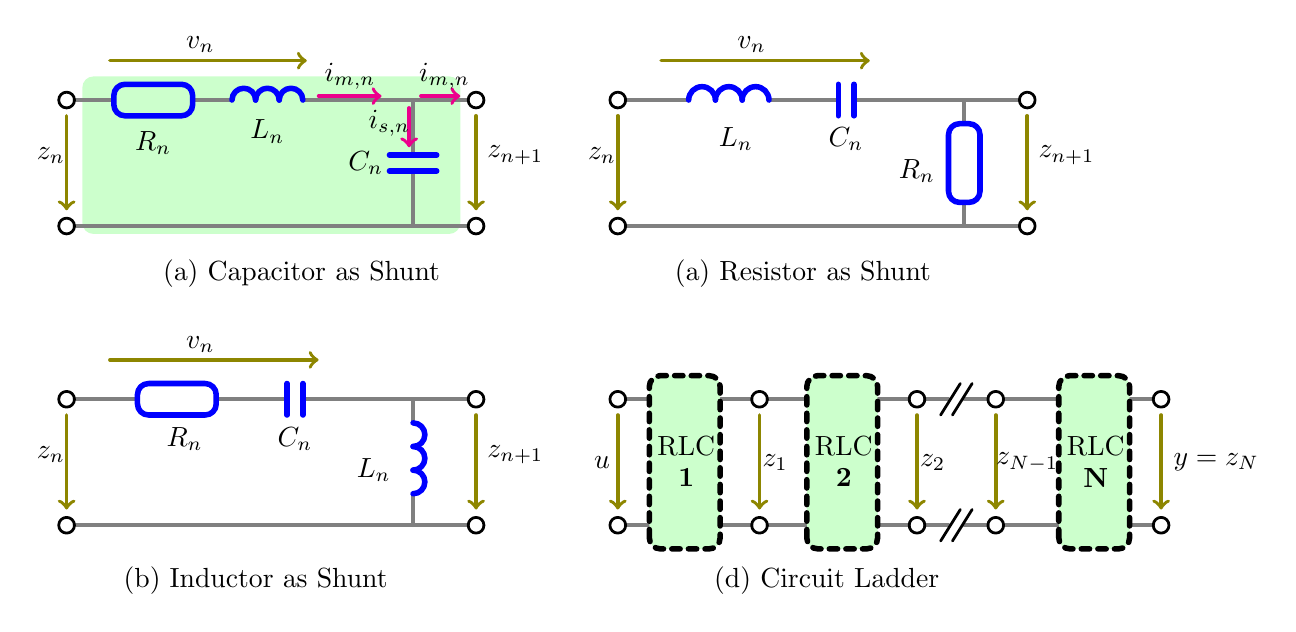
\begin{tikzpicture}[scale=1,line cap=round,line join=round,x=1.0cm,y=1.0cm]	
		\def\dxoff{7};
		\def\dyoff{3.8};
		
		\fill[color=green!20,opacity=10, rounded corners] (0.1,-1.7) rectangle (4.9,0.3);
		
		\draw[line width=1.3, color=gray] (0,0) -- (0.5,0);
		\draw[line width=1.3, color=gray] (1.5,0) -- (2.0,0);
		\draw[line width=1.3, color=gray] (2.9,0) -- (5.0,0);
		\draw[line width=1.3, color=gray] (4.3,0) -- (4.3,-0.7);
		\draw[line width=1.3, color=gray] (4.3,-0.9) -- (4.3,-1.6);
		\draw[line width=1.3, color=gray] (0,-1.6) -- (5.,-1.6);
		
		% Connector nodes
		\draw [line width=1.0] (-0.1, 0) circle [radius = 0.1];
		\draw [line width=1.0] ( 5.1, 0) circle [radius = 0.1];
		\draw [line width=1.0] (-0.1,-1.6) circle [radius = 0.1];
		\draw [line width=1.0] ( 5.1,-1.6) circle [radius = 0.1];
		
		% Resistor
		\draw[line width=2, color=blue,rounded corners] (0.5,-0.2) rectangle (1.5,0.2);
		
		
		% Inductor
		\draw[line width=2, color=blue] (2.0,0.) arc ( 180:0:0.15);
		\draw[line width=2, color=blue] (2.3,0.) arc ( 180:0:0.15);
		\draw[line width=2, color=blue] (2.6,0.) arc ( 180:0:0.15);
		
		% Capacitor
		\draw[line width=2, color=blue]  (4.0,-0.7) -- (4.6,-0.7);
		\draw[line width=2, color=blue]  (4.0,-0.9) -- (4.6,-0.9);
		
		\node at ( 1., -0.55) {$R_{n}$};
		\node at ( 2.45, -0.4) {$L_{n}$};
		\node at ( 3.7, -0.8) {$C_{n}$};
		
		
		% Currents
		\draw [->, line width=1.3, color=magenta] (3.1,0.05) -- (3.9,0.05);
		\draw [->, line width=1.3, color=magenta] (4.4,0.05) -- (4.9,0.05);
		\draw [->, line width=1.3, color=magenta] (4.25,-0.1) -- (4.25,-0.6);
		\node at (3.5, 0.3) {$i_{m,n}$};
		\node at (4.7, 0.3) {$i_{m,n}$};
		\node at (4.0, -0.3) {$i_{s,n}$};
		
		% Voltages
		\draw [->, line width=1.3, color=olive]	(-0.1, -0.2) -- (-0.1, -1.4);
		\draw [->, line width=1.3, color=olive]	( 5.1, -0.2) -- ( 5.1, -1.4);
		\draw [->, line width=1.3, color=olive]	( 0.45, 0.5) -- ( 2.95, 0.5);
		\node at (-0.3, -0.7) {$z_{n}$};
		\node at ( 5.6, -0.7)  {$z_{n+1}$};
		\node at ( 1.6, 0.7) {$v_{n}$};
		
		\node[right] at (1.0, -2.2) {(a) Capacitor as Shunt};
		
		
		
		%%% 2. Circuit: Resistor as Shunt %%%%%
		%%% 2. Circuit: Resistor as Shunt %%%%%
		%%% 2. Circuit: Resistor as Shunt %%%%%
		\draw[line width=1.3, color=gray] (\dxoff+0,0) -- (\dxoff+0.8,0);
		\draw[line width=1.3, color=gray] (\dxoff+1.82,0) -- (\dxoff+2.7,0);
		\draw[line width=1.3, color=gray] (\dxoff+2.9,0) -- (\dxoff+5.0,0);
		\draw[line width=1.3, color=gray] (\dxoff+4.3,0) -- (\dxoff+4.3,-0.3);
		\draw[line width=1.3, color=gray] (\dxoff+4.3,-1.3) -- (\dxoff+4.3,-1.6);
		\draw[line width=1.3, color=gray] (\dxoff+0,-1.6) -- (\dxoff+5.0,-1.6);
		
		
		% Nodes
		\draw [line width=1.0] (\dxoff-0.1, 0) circle [radius = 0.1];
		\draw [line width=1.0] (\dxoff+5.1, 0) circle [radius = 0.1];
		\draw [line width=1.0] (\dxoff-0.1,-1.6) circle [radius = 0.1];
		\draw [line width=1.0] (\dxoff+5.1,-1.6) circle [radius = 0.1];
		
		% Voltages
		\draw [->, line width=1.3, color=olive]	(\dxoff -0.1, -0.2) -- (\dxoff -0.1, -1.4);
		\draw [->, line width=1.3, color=olive]	(\dxoff +5.1, -0.2) -- (\dxoff +5.1, -1.4);
		\draw [->, line width=1.3, color=olive]	(\dxoff +0.45, 0.5) -- (\dxoff +3.1, 0.5);
		
		\node at (\dxoff -0.3, -0.7) {$z_{n}$};
		\node at (\dxoff+ 5.6, -0.7)  {$z_{n+1}$};
		\node at (\dxoff+ 1.6, 0.7) {$v_{n}$};
		
		% Inductor
		\draw[line width=2, color=blue] (\dxoff+0.8, 0) arc ( 180:0:0.17);
		\draw[line width=2, color=blue] (\dxoff+1.14, 0) arc ( 180:0:0.17);
		\draw[line width=2, color=blue] (\dxoff+1.48, 0) arc ( 180:0:0.17);
		
		% Capacitor
		\draw[line width=2, color=blue] (\dxoff+2.7,-0.2) -- (\dxoff+2.7,0.2);
		\draw[line width=2, color=blue] (\dxoff+2.9,-0.2) -- (\dxoff+2.9,0.2);
		
		% Resistor
		\draw[line width=2, color=blue,rounded corners] (\dxoff+4.1,-0.3) rectangle (\dxoff+4.5,-1.3);
		
		\node at (\dxoff+ 1.4, -0.5) {$L_{n}$};
		\node at (\dxoff+ 2.8, -0.5) {$C_{n}$};
		\node at (\dxoff+ 3.7, -0.9) {$R_{n}$};
		
		\node[right] at (\dxoff+0.5, -2.2) {(a) Resistor as Shunt};
		
		%%% 2. Circuit: Inductor as Shunt %%%%%
		%%% 2. Circuit: Inductor as Shunt %%%%%
		%%% 2. Circuit: Inductor as Shunt %%%%%
		
		\draw[line width=1.3, color=gray] (  0, 0-\dyoff) -- (0.8,0-\dyoff);
		\draw[line width=1.3, color=gray] (1.8, 0-\dyoff) -- (2.7,0-\dyoff);
		\draw[line width=1.3, color=gray] (2.9, 0-\dyoff) -- (5.0,0-\dyoff);
		\draw[line width=1.3, color=gray] (4.3, 0-\dyoff) -- (4.3,-0.3-\dyoff);
		\draw[line width=1.3, color=gray] (4.3,-1.2-\dyoff) -- (4.3,-1.6-\dyoff);
		
		\draw[line width=1.3, color=gray] (  0,-1.6-\dyoff) -- (5.0,-1.6-\dyoff);
		
		% Nodes
		\draw [line width=1.0] (-0.1, 0-\dyoff) circle [radius = 0.1];
		\draw [line width=1.0] ( 5.1, 0-\dyoff) circle [radius = 0.1];
		\draw [line width=1.0] (-0.1,-1.6-\dyoff) circle [radius = 0.1];
		\draw [line width=1.0] ( 5.1,-1.6-\dyoff) circle [radius = 0.1];
		
		% Voltages
		\draw [->, line width=1.3, color=olive]	(-0.1, -0.2-\dyoff) -- (-0.1, -1.4-\dyoff);
		\draw [->, line width=1.3, color=olive]	( 5.1, -0.2-\dyoff) -- ( 5.1, -1.4-\dyoff);
		\draw [->, line width=1.3, color=olive]	( 0.45, 0.5-\dyoff) -- ( 3.1, 0.5-\dyoff);
		
		\node at (-0.3, -0.7-\dyoff) {$z_{n}$};
		\node at ( 5.6, -0.7-\dyoff)  {$z_{n+1}$};
		\node at ( 1.6, 0.7-\dyoff) {$v_{n}$};
		
		% Resistor
		\draw[line width=2, color=blue,rounded corners] (0.8,-0.2-\dyoff) rectangle (1.8,0.2-\dyoff);
		
		% Capacitor
		\draw[line width=2, color=blue] (2.7,-0.2-\dyoff) -- (2.7,0.2-\dyoff);
		\draw[line width=2, color=blue] (2.9,-0.2-\dyoff) -- (2.9,0.2-\dyoff);
		
		% Inductor
		\draw[line width=2, color=blue] (4.3,-0.3-\dyoff) arc ( 90:-90:0.15);
		\draw[line width=2, color=blue] (4.3,-0.6-\dyoff) arc ( 90:-90:0.15);
		\draw[line width=2, color=blue] (4.3,-0.9-\dyoff) arc ( 90:-90:0.15);
		
		
		\node at ( 1.4, -0.5-\dyoff) {$R_{n}$};
		\node at ( 2.8, -0.5-\dyoff) {$C_{n}$};
		\node at ( 3.8, -0.9-\dyoff) {$L_{n}$};
		
		\node[right] at (0.5, -2.3-\dyoff) {(b) Inductor as Shunt};	
		
		
		%%%%% Cascaded RLC %%%%%%%%%%%%
		%%%%% Cascaded RLC %%%%%%%%%%%%
		%%%%% Cascaded RLC %%%%%%%%%%%%
		
		\draw[line width=1.3, color=gray] (\dxoff+0  , 0-\dyoff) -- (\dxoff+0.3, 0-\dyoff);
		\draw[line width=1.3, color=gray] (\dxoff+0  ,-1.6-\dyoff) -- (\dxoff+0.3,-1.6-\dyoff);
		\draw[line width=1.3, color=gray] (\dxoff+1.2, 0-\dyoff) -- (\dxoff+1.6, 0-\dyoff);
		\draw[line width=1.3, color=gray] (\dxoff+1.2,-1.6-\dyoff) -- (\dxoff+1.6,-1.6-\dyoff);
		\draw[line width=1.3, color=gray] (\dxoff+1.8, 0-\dyoff) -- (\dxoff+2.3, 0-\dyoff);
		\draw[line width=1.3, color=gray] (\dxoff+1.8,-1.6-\dyoff) -- (\dxoff+2.3,-1.6-\dyoff);
		\draw[line width=1.3, color=gray] (\dxoff+3.2, 0-\dyoff) -- (\dxoff+3.6, 0-\dyoff);
		\draw[line width=1.3, color=gray] (\dxoff+3.2,-1.6-\dyoff) -- (\dxoff+3.6,-1.6-\dyoff);			
		\draw[line width=1.3, color=gray] (\dxoff+3.8, 0-\dyoff) -- (\dxoff+4.1, 0-\dyoff);
		\draw[line width=1.3, color=gray] (\dxoff+3.8,-1.6-\dyoff) -- (\dxoff+4.1,-1.6-\dyoff);			
		\draw[line width=1.3, color=gray] (\dxoff+4.3, 0-\dyoff) -- (\dxoff+4.6, 0-\dyoff);
		\draw[line width=1.3, color=gray] (\dxoff+4.3,-1.6-\dyoff) -- (\dxoff+4.6,-1.6-\dyoff);
		\draw[line width=1.3, color=gray] (\dxoff+4.8, 0-\dyoff) -- (\dxoff+5.5, 0-\dyoff);
		\draw[line width=1.3, color=gray] (\dxoff+4.8,-1.6-\dyoff) -- (\dxoff+5.5,-1.6-\dyoff);
		\draw[line width=1.3, color=gray] (\dxoff+6.4, 0-\dyoff) -- (\dxoff+6.7, 0-\dyoff);
		\draw[line width=1.3, color=gray] (\dxoff+6.4,-1.6-\dyoff) -- (\dxoff+6.7,-1.6-\dyoff);	
		
		\draw [line width=1.0] (\dxoff+-0.1, 0-\dyoff) circle [radius = 0.1];
		\draw [line width=1.0] (\dxoff+-0.1,-1.6-\dyoff) circle [radius = 0.1];
		
		\draw [line width=1.0] (\dxoff+1.7, 0-\dyoff) circle [radius = 0.1];
		\draw [line width=1.0] (\dxoff+ 1.7,-1.6-\dyoff) circle [radius = 0.1];
		
		\draw [line width=1.0] (\dxoff+3.7, 0-\dyoff) circle [radius = 0.1];
		\draw [line width=1.0] (\dxoff+ 3.7,-1.6-\dyoff) circle [radius = 0.1];
		
		\draw [line width=1.0] (\dxoff+ 4.7, 0-\dyoff) circle [radius = 0.1];
		\draw [line width=1.0] (\dxoff+ 4.7,-1.6-\dyoff) circle [radius = 0.1];
		
		\draw [line width=1.0] (\dxoff+ 6.8, 0-\dyoff) circle [radius = 0.1];
		\draw [line width=1.0] (\dxoff+ 6.8,-1.6-\dyoff) circle [radius = 0.1];
		
		\draw [line width=1.0] (\dxoff+4,   -0.2-\dyoff) -- (\dxoff+4.25, 0.2-\dyoff);	
		\draw [line width=1.0] (\dxoff+4.15,-0.2-\dyoff) -- (\dxoff+4.4 , 0.2-\dyoff);	
		\draw [line width=1.0] (\dxoff+4,   -1.8-\dyoff) -- (\dxoff+4.25,-1.4-\dyoff);	
		\draw [line width=1.0] (\dxoff+4.15,-1.8-\dyoff) -- (\dxoff+4.4 ,-1.4-\dyoff);		
		
		\draw[dashed,line width=2,rounded corners, fill=green!20] (\dxoff+0.3,-1.9-\dyoff) rectangle (\dxoff+1.2,0.3-\dyoff);
		\draw[dashed,line width=2,rounded corners, fill=green!20] (\dxoff+2.3,-1.9-\dyoff) rectangle (\dxoff+3.2,0.3-\dyoff);
		\draw[dashed,line width=2,rounded corners, fill=green!20] (\dxoff+5.5,-1.9-\dyoff) rectangle (\dxoff+6.4,0.3-\dyoff);
		
		\node at (\dxoff+0.77,-0.6-\dyoff) {RLC};
		\node at (\dxoff+0.77,-1.0-\dyoff) {\textbf{1}};
		
		\node at (\dxoff+2.77,-0.6-\dyoff) {RLC};
		\node at (\dxoff+2.77,-1.0-\dyoff) {\textbf{2}};
		
		\node at (\dxoff+5.97,-0.6-\dyoff) {RLC};
		\node at (\dxoff+5.97,-1.0-\dyoff) {\textbf{N}};
		
		% Voltages
		\draw [->, line width=1.3, color=olive]	(\dxoff+-0.1, -0.2-\dyoff) -- (\dxoff+-0.1, -1.4-\dyoff);
		\draw [->, line width=1.3, color=olive]	(\dxoff+ 1.7, -0.2-\dyoff) -- (\dxoff+ 1.7, -1.4-\dyoff);
		\draw [->, line width=1.3, color=olive]	(\dxoff+ 3.7, -0.2-\dyoff) -- (\dxoff+ 3.7, -1.4-\dyoff);
		\draw [->, line width=1.3, color=olive]	(\dxoff+ 4.7, -0.2-\dyoff) -- (\dxoff+ 4.7, -1.4-\dyoff);
		\draw [->, line width=1.3, color=olive]	(\dxoff+ 6.8, -0.2-\dyoff) -- (\dxoff+ 6.8, -1.4-\dyoff);
		\node at (\dxoff+-0.3, -0.8-\dyoff) {$u$};
		\node at (\dxoff+ 1.9, -0.8-\dyoff) {$z_{1}$};
		\node at (\dxoff+ 3.9, -0.8-\dyoff) {$z_{2}$};
		\node at (\dxoff+ 5.1, -0.8-\dyoff) {$z_{N-1}$};
		\node at (\dxoff+ 7.5, -0.8-\dyoff)  {$y=z_{N}$};
		
		\node[right] at (\dxoff+1.0, -2.3-\dyoff) {(d) Circuit Ladder};
		
	\end{tikzpicture}
	\caption{Considered types of RLC circuits (a-c) and a Ladder of such circuits (d). The voltage at the last shunt is the output, $z_{n} = y$.}
	\label{fig:cascaded_rlc_circuits}
	
\end{figure*}


\begin{table}[hb!]
	\centering
	\renewcommand{\arraystretch}{1.3}
	\fontfamily{ppl}\selectfont
	\begin{tabular}{lll}
		\toprule
		\textbf{Sym.} & \textbf{Explanation}  & \textbf{Domain}  \\
		\midrule
		$u$ & Input voltage & $[0,T] \rightarrow \mathbb{R}$ \\
		$y$ & Output voltage & $[0,T] \rightarrow \mathbb{R}$ \\
		$v_{n}$ & Voltage at main branch & $[0,T] \rightarrow \mathbb{R}$ \\
		$z_{n}$ & Voltage at shunt & $[0,T] \rightarrow \mathbb{R}$ \\
		$i_{m,n}$ & Current through main branch & $[0,T] \rightarrow \mathbb{R}$ \\
		$i_{s,n}$ & Current through shunt & $[0,T] \rightarrow \mathbb{R}$ \\
		$R_{n}$, $L_{n}$, $C_{n}$ & Resistor, Inductor, Capacitor & $\mathbb{R}_{>0} \setminus \{\infty\}$ \\
		\bottomrule
	\end{tabular}
	\caption{Nomenclature of electrical states and quantities.}
	\label{table:el_symbols_explanation}
\end{table}

We begin the modeling with a single circuit of a ladder and demonstrate afterwards how to scale this approach for a specific RLC ladder. In our modeling approach, we consider nominal electronic components, i.e. a resistor has only a pure resistance without inductance or capacitance; and we assume a voltage source, which can supply an arbitrary signal. The voltages, currents and the quantities of the electrical components are noted in Table \ref{table:el_symbols_explanation}. The currents and voltages are functions of time, e.g. $u: [0,T] \rightarrow\mathbb{R}$ with final time $T>0$, while the quantities 	$R_{n}$, $L_{n}$ and $C_{n}$ are constant. We summarize the voltages at the shunt as 
\begin{equation}
	z = \left[z_{1}, z_{2}, \ldots, z_{N}\right]^{\top} \label{eq:z_voltages_shunt}
\end{equation}	
and we consider the voltage at the last shunt as the output voltage $y(t) = z_{N}(t)$. We consider the currents and voltages to be sufficiently smooth, e.g. twice smoothly differentiable $i_{n}, v_{n}, z_{n} \in \mathcal{C}^{2}([0,T])$, and integrable, e.g. $\int_{0}^{T} i_{n}(\tau) d\tau < \infty$. According to Kirchhoff's voltage law, the $n$-th shunt voltage is identified by
\begin{equation}
	z_{n}(t) = v_{n+1}(t) + z_{n+1}(t) = \left[\sum_{k=n+1}^{N} v_{k}(t)\right] + z_{N} \label{eq:kirchhoff_voltage}
\end{equation}
and the input voltage in the first circuit is $z_{0} = u(t)$. As a ladder is a cascade of parallel circuits, the currents split up to the subsequent circuit $n+1$ and the shunt as
\begin{equation}
	i_{m,n}(t) =~ i_{m,n+1}(t) + i_{s,n}(t) ~=~ \sum_{k=n}^{N} i_{s,k}(t) \label{eq:kirchhoff_current}
\end{equation}
with the current in the final circuit $i_{m,N}(t) = i_{s,N}(t)$. We know that the ideal voltage $x:[0,\infty) \rightarrow \mathbb{R}$ across the electrical components is stated as 
\begin{align*}
	\text{Resistor:} \quad x(t) =&~ R ~ i(t) ~\text{,}\\
	\text{Inductor:} \quad x(t) =&~ L ~ \partial_{t} i(t) ~\text{,}\\
	\text{Capacitor:} \quad x(t) =&~ \frac{1}{C} ~ \int_{0}^{t} i(\tau) d\tau \text{.}
\end{align*}
These identities and compositions according to Eq. \eqref{eq:kirchhoff_voltage} are modeled as linear operator mappings 
\begin{equation*}
	\mathcal{F}\{i\}(t) = c_{0} ~ i(t) +  c_{1}~ \partial_{t} i(t) +  c_{2}~ \int_{0}^{t} i(\tau) d\tau 
\end{equation*}
where we distinguish these mappings for the main branch and shunt as
\begin{equation}
	v_{n}(t) = \mathcal{F}_{m,n} \left\{i_{m,n}\right\}(t) ~ \text{,} \quad 
	z_{n}(t) = \mathcal{F}_{s,n} \left\{i_{s,n}\right\}(t) \text{.} \label{eq:operator_maps}
\end{equation}
Subsequently, we apply the Kirchhoff laws and the operator mappings on the considered types of RLC ladders, see Fig. \ref{fig:cascaded_rlc_circuits}, in order to derive the systems of linear ordinary differential equations.



\subsection{RLC Ladder with Capacitor at Shunt}

In the first case, see Fig. \ref{fig:cascaded_rlc_circuits} (a), the voltage in the main branch with a resistor and an inductor is stated as
\begin{align}
	v_{n}(t) =&~ R_n i_{m,n}(t) + L_n \partial_{t} i_{m,n}(t) \nonumber \\ 
	=&~ (R_{n} + L_{n}\partial_{t}) ~ i_{m,n}(t) = \mathcal{F}_{m,n} \left\{i_{m,n}\right\}(t) \\ 
	=&~ \left[R_{n} + L_{n}\partial_{t}\right] ~ \sum_{k=n}^{N} i_{s,k}(t) \text{,} \label{eq:rlc_cap_volt_r_l}
\end{align}
and the shunt voltage is noted as
\begin{equation}
	z_{n}(t) =~ \frac{1}{C_{n}} \int_{0}^{t} i_{s,n}(\tau) d\tau ~~= \mathcal{F}_{s,n} \left\{i_{s,n}\right\}(t) \text{.} \label{eq:rlc_cap_volt_c}
\end{equation}
We compute the inverse operator mapping of Eq. \eqref{eq:rlc_cap_volt_c} as 
\begin{equation*}
	i_{s,n}(t) = \mathcal{F}_{s,n}^{-1} \left\{z_{n}\right\}(t) = C_{n} \partial_{t} z_{n}	
\end{equation*}
and insert it in Eq. \eqref{eq:rlc_cap_volt_r_l} to yield
\begin{align}
	v_{n}(t) =&~  \left[R_{n} + L_{n}\partial_{t}\right] ~ \sum_{k=n}^{N} C_{k} ~ \partial_{t} z_{k}(t) \nonumber \\
	=&~  \sum_{k=n}^{N} \left[ R_{n} ~  C_{k} ~  \partial_{t} + L_{n} ~  C_{k} ~ \partial^2_{t}\right] z_{k}(t) \label{eq:rlc_cap_volt_r_l_2}
\end{align}
We consider Kirchhoff's voltage law \eqref{eq:kirchhoff_voltage} with the voltage in main branch \eqref{eq:rlc_cap_volt_r_l_2} and so we calculate the shunt voltage for the $n$-th circuit, $n\in\{2,\ldots,N\}$ as the differential equation
\begin{align}
	0 =&~ \sum_{k=n}^{N} \left[ L_{n} C_{k} ~ \partial_{t}^2 z_{k}(t) + R_{n} C_{k} ~ \partial_{t} z_{k}(t)  \right] \nonumber \\
	&\qquad  + z_{n}(t) - z_{n-1}(t) \text{.} \label{eq:rl-c_shunt_ode_n}
\end{align}
For the first circuit of the ladder, we have $u(t) = z_{0}(t)$ and so we note
\begin{equation}
	u(t) =~ \sum_{k=1}^{N} \left[ L_{1} C_{k} ~ \partial_{t}^2 z_{k}(t) + R_{1} C_{k} ~ \partial_{t} z_{k}(t)  \right] + z_{1}(t) \text{.} \label{eq:rl-c_shunt_ode_0}
\end{equation}



\subsection{Resistor as Shunt}
In the second case, see Fig. \ref{fig:cascaded_rlc_circuits} (b), we have an inductor and a capacitor in the main branch and a resistor as shunt. Hence, we note the voltages as 
\begin{align} % Type LC-R
	v_{n}(t) =&~ L_n ~ \partial_{t} i_{m,n}(t) + \frac{1}{C_{n}} \int_{0}^{t} i_{m,n}(\tau) d\tau \nonumber \\
	=&~ \mathcal{F}_{m,n} \left\{i_{m,n}\right\}(t) \qquad\text{and} \label{eq:lc-r_volt_main} \\
	z_{n}(t) =&~ R_n ~ i_{s,n}(t)  = \mathcal{F}_{s,n} \left\{i_{s,n}\right\}(t) \text{.} \label{eq:lc-r_volt_shunt}
\end{align}
We differentiate both sides of Eq. \eqref{eq:lc-r_volt_main} and we apply Eq. (\ref{eq:kirchhoff_current}, \eqref{eq:lc-r_volt_shunt}) to obtain
\begin{align*}
	\partial_{t} v_{n}(t) =&~ \left[L_n \partial_{t}^2 + \frac{1}{C_{n}}\right] i_{m,n}(t) \\
	=&~ \left[L_n \partial_{t}^2 + \frac{1}{C_{n}}\right] \left[  \sum_{k=n}^{N} i_{s,k}(t)  \right] \\
	=&~ \left[L_n \partial_{t}^2 + \frac{1}{C_{n}}\right] \left[  \sum_{k=n}^{N} \frac{z_{k}(t)}{R_{k}} \right] \text{.}
\end{align*}
We evaluate the Kirchhoff voltage law \eqref{eq:kirchhoff_voltage} and we  note the differential equation of the $n$-th circuit 
for  $k\in\{2,\ldots,N\}$ as 
\begin{align}
	0 =&~ \sum_{k=n}^{N} \left[ \frac{L_{n}}{R_{k}} ~ \partial_{t}^2 z_{k}(t) + \frac{z_{k}(t)}{R_{k}~C_{n}} \right] \nonumber \\
	&\qquad   + \partial_{t} \left[z_{n}(t) - z_{n-1}(t)\right] \label{eq:lc-r_shunt_ode_n}
\end{align}
for $n\in\{2,\ldots,N\}$, and for $n=1$ we have
\begin{equation}
	\partial_{t} u(t) =~ \sum_{k=1}^{N} \left[ \frac{L_{1}}{R_{k}} ~ \partial_{t}^2 z_{k}(t) + \frac{z_{k}(t)}{R_{k}~C_{1}} \right] + \partial_{t} z_{1}(t) \text{.} \label{eq:lc-r_shunt_ode_0}
\end{equation}


\subsection{Inductor as Shunt}
In case of the third circuit type, see Fig. \ref{fig:cascaded_rlc_circuits} (c), we note the voltages as 
\begin{align}
	v_{n}(t) =&~ R_n ~ i_{m,n}(t) + \frac{1}{C_{n}} \int_{0}^{t} i_{m,n}(\tau) d\tau \text{,} \label{eq:rc-l_volt_main}  \\ 
	z_{n}(t) =&~ L_n ~ \partial_{t} i_{s,n}(t) \text{.} \label{eq:rc-l_volt_shunt}
\end{align}
We differentiate Eq. \eqref{eq:rc-l_volt_main} two times and we insert $\partial_{t} i_{s,n}(t)$ from Eq. \eqref{eq:rc-l_volt_shunt}. Hence, we yield the identity
\begin{align*}
	\partial_{t}^2 v_{n}(t) =&~ \left[R_n ~ \partial_{t} + \frac{1}{C_{n}} \right] \partial_{t}  i_{m,n}(t) \\
	=&~ \left[R_n ~ \partial_{t} + \frac{1}{C_{n}} \right]  \left[ \sum_{k=n}^{N} \frac{z_{k}(t)}{L_{k}}  \right] \text{.}
\end{align*}
In a analog way as before, we note the differential equation of the $n-th$ circuit as
\begin{align}
	0 =&~  \partial_{t}^2 \left[z_{n}(t) - z_{n-1}(t)\right] \nonumber \\
	&\quad + \sum_{k=n}^{N} \left[ \frac{R_{n}}{L_{k}}~\partial_{t} z_{k}(t) + \frac{z_{k}(t)}{L_{k}~C_{n}} \right] \label{eq:rc-l_shunt_ode_n}
\end{align}
and for the first circuit, we note
\begin{equation}
	\partial_{t}^2 u(t) =~  \partial_{t}^2 z_{1}(t) + \sum_{k=n}^{N} \left[ \frac{R_{1}}{L_{k}}~\partial_{t} z_{k}(t) + \frac{z_{k}(t)}{L_{k}~C_{1}} \right] \text{.} \label{eq:rc-l_shunt_ode_0}
\end{equation}
